
% to choose your degree
% please un-comment just one of the following
\documentclass[bsc,frontabs,twoside,singlespacing,parskip,deptreport]{infthesis}     % for BSc, BEng etc.
% \documentclass[minf,frontabs,twoside,singlespacing,parskip,deptreport]{infthesis}  % for MInf
\usepackage{graphicx}
\usepackage{hyperref}
\begin{document}

\title{Microbenchmarking Intel Knights Landing}

\author{Alexander Wilson}
 
\course{Computer Science}  

\project{4th Year Project Report}

\date{\today} 

\abstract{
@TODO
}

\maketitle

\section*{Acknowledgements}
@TODO 

\tableofcontents

%\pagenumbering{arabic}


\chapter{Introduction}
\section{Project Motivation}
With processors becoming increasingly complex, and the need for large data processing, hardware manufacturers like Intel are producing new and different processors to tackle different problems, using new or different architectural designs. It is interesting to investigate the design choices made, and think about the different potential applications of new architectural designs.

\section{Project Overview}
The goal of this project is to evaluate the performance of Intel's 2nd Generation Xeon Phi processor's(code-named Knights Landing) memory system. The processor has a complex and interesting memory system, including new memory modules relative to predecessors. The project will include measuring the latencies of accessing the different memory components and bandwidths between them.


\chapter{Background}
\section{Computer Architecture}
This section will cover design features present in modern processors that are relevant to the scope of this project, specifically in understanding how benchmarks are written.

\subsection{Pipelining}
Pipelining is a technique used in almost all modern processors to commit more instructions per cycle. The technique involves splitting an instruction into stages, and then once any given stage has completed, a new instruction can enter that stage. For example, we could consider a processor to process instructions over 5 stages:
\begin{enumerate}
    \item{{\bf \texttt{IF} - Instruction Fetch} \\ The instruction at the program counter(PC) is fetched from memory, and the PC is incremented.}
    \item{{\bf \texttt{ID} - Instruction Decode} \\ The fetched instruction is decoded, and required values are fetched from general purpose Registers.}
    \item{{\bf \texttt{EXE} - Execution} \\ The arithmetic and logic operations are computed. This includes computation of addresses. }
    \item{{\bf \texttt{MEM} - Memory Access/Branch Completion} \\ Memory is accessed if required.}
    \item{{\bf \texttt{WB} - Write Back} \\ Results of execution are written back to general purpose Registers}
\end{enumerate}
Splitting instruction execution into stages like the above model, it allows the processor to reallocate a given stages resources to a new instruction, once the current instruction has finished using those resources. For example the processor can begin fetching the next instruction after it has finished fetching the current instruction, but before the current instruction has totally finished being executed. This means that in the ideal situation, our model can have 5 instructions in flight, and given that each stage costs one cycle, potentially committing an instruction every cycle. It is important to note that in practise, this is likely won't happen, for example complex arithmetic, such as divisions, will take multiple cycles to complete the \texttt{EXE} stage.

\subsection{Out-Of-Order Execution}
Out of order execution is a technique used in processors to increase the efficiency of the pipeline. The processor can re-order instructions to make more efficient usage of the different stages. For example, if you have a complex division instruction, followed by a few simple addition instructions, the processor could push the additions into the pipeline first, and the division last, so that the pipeline doesn't halt or bottleneck at the \texttt{EXE} stage while waiting for the complex division to be calculated, leaving other instructions halted in flight behind it. Out-Of-Order execution is complex, and if the CPU were to re-order dependent instructions, it would have other systems in place to handle instruction dependencies. An example of such a dependency would be:
\begin{center}
\verb
x = a / b
\\
\verb
y = x + 5
\end{center}
Where the value of \texttt{y} cannot be calculate until the result of \texttt{x} has been calculated, and so \texttt{y = x + 5} may hang at the \texttt{ID} stage, essentially halting the pipeline. However mitigations and workarounds to tackle instruction dependencies are out of the scope of the project, it is important to understand that modern processors may re-order instructions.


\subsection{Caching}
\subsubsection{Motivation}
Moore's Law states that the number of transistors that could be fit onto a computer chip would scale up by a factor of five, every five years. To begin with, the extra transistors on the chips were used for created logical units that could compute logical/arithmetic operations quicker, however it was soon realised that despite processors being able to process arithmetic with a latency as low as a single cycle, actually retrieving the data to perform the logical/arithmetic operations on was becoming a huge bottleneck. For example; the \texttt{EXE} stage of the pipeline could process simple addition operations in a single cycle, but retrieving the additions operands could cost a few hundred cycles to retrieve from memory, and so memory latency became a significant bottleneck in the pipeline.
\subsubsection{Solution}
The solution to this problem has not just been to throw more hardware at main memory, but to use the new transistors on chips to create a memory hierarchy that caches and pre-fetches data that is likely to be used. Most general purpose CPU's today have a two to three level cache hierarchy, with level one being the smallest and closest to the processor cores, and level 3 being the biggest. When referring to different levels of caches in a processor, \texttt{L1} is used to refer to the level one cache; likewise \texttt{L2} to refer to the level two cache.
\par
\subsubsection{Cache Behaviour}
Each processor line will have its own unique cache architecture. However it is typical for an \texttt{L1} cache to exist spatially close to a single core, and be unique to that core. Some architectures have \texttt{L2} caches unique to a core, however it is more common that the \texttt{L2} cache is shared among cores. There are two ways that caches are designed to be indexed; Direct-Mapping and Set-Associative.
\begin{itemize}
    \item{
        {\bf Direct Mapping} \\
        Each line in memory is mapped to a specific line in the cache. If memory has \texttt{M} lines, and our cache has \texttt{C} lines, where \texttt{C < M}, memory line \texttt{m} is located in the cache at line \texttt{m modulo C}\\
        This has the advantage of being quick to access, as you simply lookup the line in cache where the address you wish to read/write to would exist, and if the tag of the cache-line and your address match, you have found your data quickly. \\
        This method can incur cache thrashing, which is when useful data is evicted from the cache, for example say you have two variables in memory, and they both map to the same cache line, the cache could be evicting and replacing this line potentially many times depending on the nature of the program and its use of the variables. \\
        \\
        Figure \ref{fig:dir_map}, shows how lines in memory are mapped to one specific line in the cache.
    }
    \begin{figure}[h]
        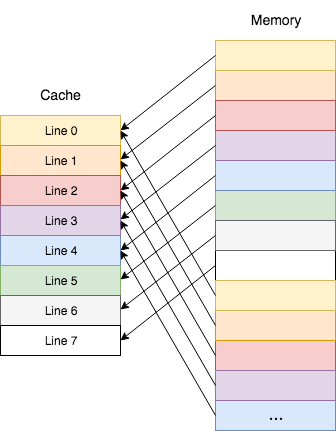
\includegraphics[width=4cm]{direct_mapped.png}
        \centering
        \caption{Direct Mapped Cache Diagram}
        \label{fig:dir_map}
    \end{figure}
    
    \item{
        {\bf Set Associative} \\
        An N-way set associative cache is a cache that is split into sets containing N lines. Therefore if we have a cache with 32 lines, and it is 4-way set associative, then our cache has 8 sets, each containing 4 lines. Memory is mapped to set-associative caches similarly to direct mapping, but instead of mapping a line in memory to a specific line in cache, it is mapped to a set in cache, and then the contents of the sets are managed using a cache replacement policy(such as least-recently used, first-in-first-out or random-replacement). This also allows for a fully-associative cache, where there is only 1 set, where all cache lines are stored/evicted based on a replacement policy. \\
        This has the advantage of dealing with cache trashing, where multiple lines can exist in the cache at the same time, that would not exist simultaneously in a Direct Mapped cache. \\
        In the case of a fully-associative cache, there is a large overhead in searching the cache for the data that you want, and so in practise, N-way set associative caches are often used in general purpose CPU's to get the best of both Direct Mapped and Fully Associative mappings. But that is not to say that there are no use-cases for Direct Mapped caches. \\
        \\
        Figure \ref{fig:set_assoc}, shows how lines in memory are mapped to one \textbf{set} in the cache. Its important to note that the items within a \textbf{set} are evicted based on the architectures chosen replacement policy. 
    }
    \begin{figure}[h]
        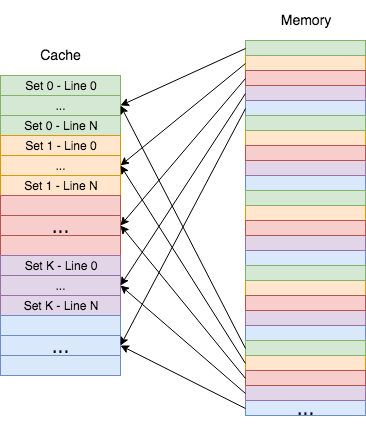
\includegraphics[width=6cm]{set_assoc.png}
        \centering
        \caption{N-way Set Associative Cache Diagram}
        \label{fig:set_assoc}
    \end{figure}
\end{itemize}

It is also important to note that a cache line can vary in size depending on architecture, but it is common for cache lines to be 64B, as it is affordable to transport 64B between caches and memory, while exploiting program spacial locality\footnote{Program Spacial Locality: Programs often access nearby memory addresses, for example incremented indexes in an array.}.

\newpage

\chapter{Understanding KNL Architecture}
This chapter will talk about what is unique about the KNL Architecture, and what needs to be known to understand how to write benchmarks.
\section{Chip Layout}
\begin{figure}[h]
    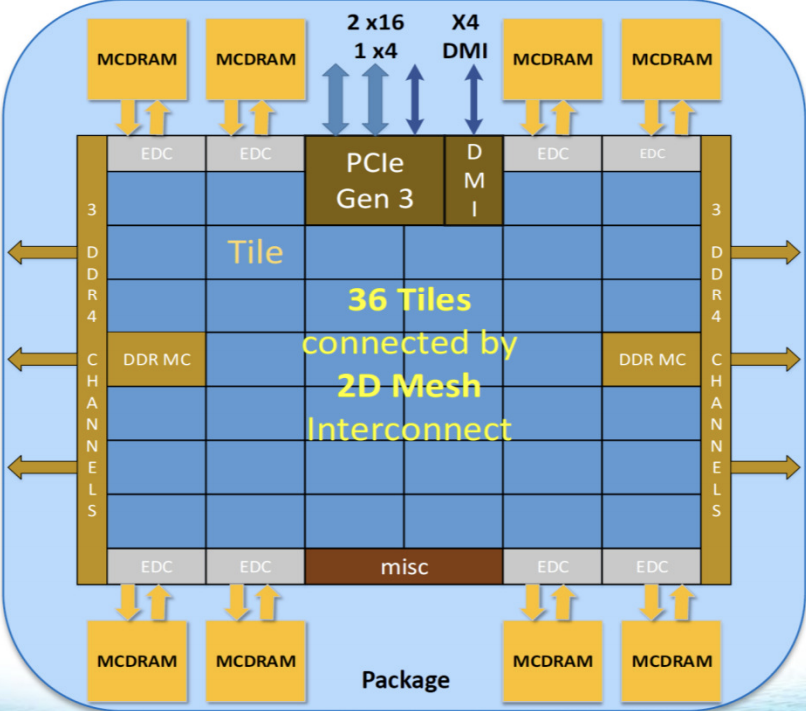
\includegraphics[width=10cm]{KNL_Overview.png}
    \centering
    \caption{KNL Chip Layout}
    \protect\cite{intel_pres}
    \label{fig:chip_overview}
\end{figure}
Figure \ref{fig:chip_overview}, shows a top-down view of the architecture of the KNL chip. The chip is a mesh of 36 tiles.

\subsection{Tile}
A tile consists of:
\begin{itemize}
    \item 2 x CPU Cores:
    \begin{itemize}
        \item \texttt{32KB L1} Instruction Cache \ \ \ \ \ \ \texttt{8-way} set-associative, \texttt{64B} cache lines
        \item \texttt{32KB L1} Data Cache \ \ \ \ \ \ \ \ \ \ \ \ \ \ \ \ \texttt{8-way} set-associative, \texttt{64B} cache lines
    \end{itemize}
    
    \item 1 x L2 Cache
    \begin{itemize}
        \item Configurable \texttt{1MB} Cache shared between Cores, or \texttt{512KB} Cache per Core.
        \item \texttt{16-way} set-associative, \texttt{64B} cache lines
        \item Performs a single \texttt{read} in \texttt{1 cycle}.
        \item Performs a single \texttt{write} in \texttt{2 cycles}.
        \item L2 Cache \textbf{coherent} with all other tiles L2 Caches.
    \end{itemize}
    
    \item 1 x Caching/Home Agent
    \begin{itemize}
        \item Distributed Tag Directory to keep \texttt{L2 Caches} coherent across tiles.
    \end{itemize}
\end{itemize}
\subsection{L2 Cache}
The mesh of tiles creates a distributed \texttt{L2} Cache. This mesh is configurable in three different modes:
\begin{itemize}

    \item \textbf{All-to-All} \\
    All of the \texttt{L2} Address space uniformly distributed across all tiles. This means that any given core can access data in the \texttt{L2} Cache of any other tile. A typical miss in All-to-All mode starts with a Core missing in its \texttt{L1} Cache, it then checks its own tiles \texttt{L2} Cache, and upon missing, checks the \textbf{distributed} directory. After missing in the \textbf{distributed} directory, the request is forwarded to MCDRAM/DRAM(Depending on configuration).\\
    Most general mode, so relatively lower performance.
    
    \item \textbf{Quadrant} \\
    The Chip is divided into four virtual quadrants. Addresses are hashed to a directory in the same quadrant. This means that a core can access data in the \texttt{L2} Cache of any other tile in the same virtual quadrant. A typical miss in Quadrant mode starts with a Core missing in its \texttt{L1} Cache, it then checks its own tiles \texttt{L2} Cache, and upon missing, checks the \textbf{quadrant} directory. After missing in the \textbf{quadrant} directory, the request is forwarded to MCDRAM/DRAM(Depending on configuration).\\
    This mode has a lower latency, and higher bandwidth relative to \texttt{All-to-All}. Quadrant's are transparent to software.
    
    \item \textbf{Sub-NUMA Clustering} \\
    The Chip is divided into four quadrants. Each exposed to the OS as a seperate NUMA\footnote{NUMA: Non-Uniform Memory Access; The idea that different cores have their own physical memory.} domain. To the operating system, this looks analogous to a 4 socket Xeon(server) processor. A typical miss in Sub-NUMA mode starts with a Core missing in its \texttt{L1} Cache, it then checks the \textbf{quadrant} directory. After missing in the \textbf{quadrant} directory, the request is forwarded to MCDRAM/DRAM(Depending on configuration). \\
    This mode has the lowest latency of all three modes, due to the nature of NUMA and spacial locality, but requires software support to handle the distributed memory.
    
\end{itemize}

\subsection{MCDRAM}
The KNL Chip includes a new layer of high-bandwidth memory that is spatially close to the chip, but has a higher access latency compared to DRAM. Intel coined MCDRAM is 16GB of RAM built into the chip, with three configurable modes:

\begin{itemize}
    \item \textbf{Cache Mode} \\
    The 16GB of memory is used to cache DRAM. This is completely transparent to software, and so any memory address that doesn't exist in the \texttt{L1} or \texttt{L2} Cache's is directed to MCDRAM next. When considering access latencies, visiting MCDRAM is already more costly than visiting DRAM, but missing in MCDRAM also then requires a further lookup to main memory. This effectively means that cache mode is best used for frequently used contiguous\footnote{Contiguous Memory: Memory that exists spatially next to each other.} memory, as it can be be pulled into \texttt{L2} and \texttt{L1} Caches with less memory accesses.
    
    \item \textbf{Flat Mode} \\
    The 16GB of memory is used to extend DRAM, essentially extending its address space. This mode requires programs to be aware of this configuration, and address memory appropriately
    
    \item \textbf{Hybrid Mode} \\
    The 16GB of memory can be used to both extend DRAM, and cache it. It can be configured to use either 25\% or 50\% of the 16GB as a DRAM Cache, with the rest extending DRAM. This has the benefit of extending DRAM, and also caching data that is frequently used.
\end{itemize}


\chapter{Writing the Microbenchmarks}
This chapter will talk about the different approaches to benchmarking latencies and bandwidths of different memory components, and tackling obstacles that would prevent accurate or reliable results.

\section{Timing Techniques}
Talk about tackling OoO Execution, pro's and con's of different timestamping techniques.
\newpage

\section{Measuring Bandwidth}
Talk about approaches considered and taken for measuring memory bandwidth
\newpage

\section{L1 Cache}
Talk about the benchmark program for measuring L1 Cache latencies.
\newpage
\section{L2 Cache}
Talk about the benchmark program for measuring L2 Cache latencies.
\newpage
\section{MCDRAM}
Talk about the benchmark program for measuring MCDRAM latencies and Bandwidth.
\newpage
\section{DRAM}
Talk about the benchmark program for measuring DRAM latencies and Bandwidth.
\newpage

\chapter{Results}
\section{Latencies}
\newpage
\section{Bandwidths}
\newpage

\chapter{Discussion}

% \chapter{TEMP - Citations}

% Note that citations 
% (like \cite{P1} or \cite{P2})
% can be generated using {\tt BibTeX} or by using the
% {\tt thebibliography} environment. This makes sure that the
% table of contents includes an entry for the bibliography.
% Of course you may use any other method as well.

% use the following and \cite{} as above if you use BibTeX
% otherwise generate bibtem entries
\bibliographystyle{plain}
\bibliography{mybibfile}

\end{document}
